\documentclass[a4paper, 10pt]{article}
\usepackage[UTF8]{ctex}
\usepackage[vmargin=.75in,hmargin=.5in]{geometry}
\usepackage{multicol}
\usepackage{amsmath, amssymb, amsthm, bm, mathrsfs}
\allowdisplaybreaks[4] % 公式跨页 Cross-page equations
\providecommand{\abs}[1]{\left\lvert#1\right\rvert} % 绝对值 Absolute
\providecommand{\norm}[1]{\left\lVert#1\right\rVert} % 范数 Norm
\providecommand{\re}{\,\mathrm{Re}\,} % 复数的实部 Real part of complex number
\providecommand{\im}{\,\mathrm{Im}\,} % 复数的虚部 Imaginary part of complex number
\providecommand{\sgn}{\,\mathrm{sgn}\,} % 符号函数 Sign function
\providecommand{\sinc}{\,\mathrm{sinc}\,} % 辛格函数 sinc function
\providecommand{\tr}{\,\mathrm{Tr}\,} % 右矢接左矢 Contiguous ket after bra
\usepackage{graphicx}
\usepackage{subfigure}
\usepackage{url}
\begin{document}
\title{基于塑料瓶的声学相控阵}
\author{陈稼霖\and 薛加民}
\date{2021 年 1 月 10 日}
\maketitle
\begin{abstract}
细口的塑料瓶可视为一亥姆霍兹共振腔,对外界的气压驱动产生声学响应. 我们测定了空塑料瓶内不同位置以及不同剩余容积的塑料瓶瓶口的声学响应特性,并据此用不同剩余容积的塑料瓶阵列演示了声音的定向发射.
\end{abstract}

相控阵雷达是一种改变天线阵列间信号相位差来实现扫描的雷达,相较于传统雷达,相控阵雷达具有扫描效率高、范围大的优点,并且能够避免机械扫描对设备的损耗. 相控阵雷达发射和接收的信号载体是电磁波,其基本原理是电磁波在空间中的干涉效应,理论上,以声波为载波,利用相同的原理,同样可以实现信号的定向发射和接收. 本文中,我们尝试使用廉价却具有良好声学响应特性的塑料瓶作为发射声波的“天线”,演示声学版本的相控阵.

\section{塑料瓶的声学响应特性}
设计声学相控阵装置之前,我们首先测定塑料瓶的声学响应特性.

\subsection{塑料瓶的亥姆霍兹共振模型}
本实验采用的是一种容积 $V=510$ mL,瓶口内径 $d=2.2$ cm,瓶口长度 $l=2.8$ cm 的塑料瓶(图 \ref{Empty-Bottle-Acoustic-Response} (a)),我们使用亥姆霍兹共振腔模型来处理其瓶口空气柱(图 \ref{Empty-Bottle-Acoustic-Response} (a) 中红色区域的空气)的振动. 由于瓶口空气柱振动幅度很小,瓶内空气(图 \ref{Empty-Bottle-Acoustic-Response} (b) 中蓝色区域的空气)对瓶口空气柱产生的回复力正比空气柱偏离其平衡位置的位移,即视空气柱为一谐振子. 空气柱振动的周期很小,故可认为振动过程中无显著的热传导,用理想气体绝热模型可得瓶口空气柱的本征振动频率
\begin{align}
    f_0=\frac{c}{4\pi}\sqrt{\frac{\pi d^2}{Vl}},
\end{align}
其中 $c$ 为声速. 实际上在瓶口附近的空气也会随着瓶口空气柱一起振动,考虑到这一点,上式可修正为\cite{fonema.se}
\begin{align}
    \label{f0}
    f_0=\frac{c}{4\pi}\sqrt{\frac{\pi d^2}{V(l+0.3d)}}
\end{align}
在周期性变化的声压$\Delta P\exp(i2\pi ft)$的驱动下,瓶口空气柱振动方程为
\begin{align}
    \ddot{x}=-(2\pi f_0)^2x-2\gamma\dot{x}+g\Delta P\exp(i2\pi ft),
\end{align}
其中 $\gamma$ 为阻尼系数,$g$ 为表征声压与空气柱耦合程度的系数. 以上方程解得空气柱的位移
\begin{align}
    x(t)=\frac{g\Delta P}{\sqrt{[(2\pi f)^2-(2\pi f_0)^2]^2-(2\gamma\cdot 2\pi f)^2}}\exp[i(2\pi ft+\phi)],
\end{align}
其中振幅
\begin{align}
    \label{amp}
    \abs{x}=\frac{g\Delta P}{\sqrt{[(2\pi f)^2-(2\pi f_0)^2]^2-(2\gamma\cdot 2\pi f)^2}},
\end{align}
当驱动频率为共振频率$\sqrt{(2\pi f_0)^2-2\gamma^2}$时,振幅达到极大值;相位 $\phi\in(-\pi,0]$,且满足
\begin{align}
    \label{phase}
    \tan\phi=\frac{2\gamma\cdot 2\pi f}{(2\pi f)^2-(2\pi f_0)^2},
\end{align}
这意味空气柱的振动落后于驱动声压且驱动声压频率越高,落后相位越大.

如图 \ref{Empty-Bottle-Acoustic-Response} (b) 所示,我们用一小音响产生驱动声压,驻极体话筒 A 固定于瓶外以监测输入塑料瓶的声波,驻极体话筒 B 固定于瓶口稍内侧以监测塑料瓶口空气柱的振动,驻极体话筒采集得到的信号经如图 \ref{Empty-Bottle-Acoustic-Response} (c) 所示的电路放大. 用驻极体话筒 B 测得信号振幅除以驻极体话筒 A 测得信号振幅,从而消除音响产生声压振幅波动以及驻极体话筒对不同频率声波响应差异的影响,得到如图 \ref{Empty-Bottle-Acoustic-Response} (d) 所示的振幅关于驱动频率的变化曲线. 利用式 \eqref{amp} 拟合可得共振频率为 $219.3$ Hz,阻尼系数 $\gamma=17.1$ Hz,本征频率 $f_0=219.4$ Hz,与用式 \eqref{f0} 计算得到的 $251.2$ Hz 符合得较好. 用驻极体话筒 $A$ 测得信号相位减去驻极体话筒 $B$ 测得信号相位以及因声波在两个驻极体话筒间传播而导致的相位差如图 \ref{Empty-Bottle-Acoustic-Response} (e) 所示,实验数据点与利用式 \eqref{phase} 计算所得曲线符合得尚好. 这些实验数据与理论的对照说明亥姆霍兹共振腔模型可以较好地处理空塑料瓶.

\begin{figure}[h]
    \centering
    \includegraphics[width=.6\columnwidth]{Empty-Bottle-Acoustic-Response.eps}
    \caption{(a) 塑料瓶尺寸,瓶壁厚 $0.2$ cm. (b) 测量空塑料瓶声学响应实验装置,其中\textcircled{1} -- 塑料瓶,\textcircled{2} 小音箱,\textcircled{3} -- 驻极体话筒 A,\textcircled{4} -- 驻极体话筒 B,红色矩形框内 -- 驻极体话筒放大电路. (c) 驻极体话筒放大电路. (d) 空塑料瓶瓶口声学响应振幅关于驱动频率的变化关系,其中蓝色散点为实验数据,橙色曲线为按照式 \eqref{amp} 得到的拟合线. (e) 空塑料瓶声学响应相位关于驱动频率的变化关系,其中蓝色散点为实验数据,橙色曲线为式 \eqref{phase} 代入(d) 中得到的本征频率和阻尼系数计算所得理论相位.}
    \label{Empty-Bottle-Acoustic-Response}
\end{figure}

\subsection{空塑料瓶不同位置的声学响应特性}
讨论塑料瓶对外加声压驱动的响应,除瓶口处空气柱的振动,还应当考虑塑料瓶内各处空气的振动情况. 如图 \ref{Empty-Bottle-Acoustic-Response-Distribution} (a) 所示,我们将驻极体话筒 B 固定于一根细木杆上沿中轴线插入塑料瓶,测量了塑料瓶不同深度处共振频率、阻尼系数(图 \ref{Empty-Bottle-Acoustic-Response-Distribution} (b))和共振振幅、相位(图 \ref{Empty-Bottle-Acoustic-Response-Distribution} (c)). 随着深入塑料瓶内部,共振频率没有发生显著变化. 阻尼系数在瓶口附近有一极大值,进入瓶内后迅速减小且随着深度不再有明显变化. 随着深入塑料瓶内,共振时的振幅先显著增大后达到相对稳定,而共振时的相位落后先显著增大,达到近$\pi/2$后保持相对稳定. 这说明声波在由瓶口进入瓶内时会遭遇较大的阻抗不匹配而损失较多能量,而进入塑料瓶内后可以较为自由地传播,瓶口和瓶深处的空气作为一整体共同振动,但由于各地阻尼系数的差异存在相位的延迟. 这也提示我们在瓶口处测量时需要将驻极体话筒适当伸入瓶口以提高信噪比,且需要固定驻极体话筒的位置以排除深度的影响.

\begin{figure}[h]
    \centering
    \includegraphics[width=.6\columnwidth]{Empty-Bottle-Acoustic-Response-Distribution.eps}
    \caption{(a) 测量空塑料瓶不同位置处声学响应的实验装置,其中驻极体话筒 B 固定在一根细木杆上沿中轴线插入塑料瓶. (b) 空塑料瓶中轴线上不同深度处共振频率和阻尼系数,其中深度为正代表驻极体话筒在内,为负代表驻极体话筒在瓶外. (c) 空塑料瓶中轴线上不同深度处共振振幅和相位.}
    \label{Empty-Bottle-Acoustic-Response-Distribution}
\end{figure}

\subsection{不同剩余容积的塑料瓶的声学响应特性}
相控阵雷达需要调节阵列中各天线的信号的相位之差,此处我们可以根据式 \eqref{f0} 调节塑料瓶内剩余容积而改变本征频率 $f_0$,进而根据式 \eqref{phase} 引起相位的改变. 如图 \ref{Bottle-With-Water} (a) 我们采用向塑料瓶内加入不同体积的水的方式改变塑料瓶的剩余容积,进而测定了在不同剩余容积情况下的本征频率,如图 \ref{Bottle-With-Water} 所示,实验测得的本征频率与式 \eqref{f0} 计算得到的理论值随着塑料瓶剩余容积的变化趋势基本一致,但总是略小于计算值,这是因为受外界气压驱动不止塑料瓶口出的空气柱,还有瓶口附近的部分空气.

\begin{figure}[h]
    \centering
    \includegraphics[width=.6\columnwidth]{Bottle-With-Water.eps}
    \caption{(a) 测量加入不同体积的水的塑料瓶的声学响应. (b) 塑料瓶本征频率 $f_0$ 随着剩余容积 $V$ 的变化关系,其中蓝色散点为实验数据,橙色曲线为根据式 \eqref{f0} 计算得到的本征频率.}
    \label{Bottle-With-Water}
\end{figure}

\section{基于塑料瓶的声学相控阵}
如图 \ref{Phased-Bottle-Array} (a) 所示,我们将两组 $3\times 3$ 个塑料瓶分别置于小音响对称的两侧 $\pm\delta z=\pm 25.0$ cm 处,其中小音箱以 $330$ Hz 频率发声,两组塑料瓶先均加水调节至共振频率为 $330$ Hz,然后从一组塑料瓶中抽水至另一组塑料瓶,最终使两组塑料瓶在以 $330$ Hz 振动时相位差 $\pi/2$,将驻极体话筒置于距离音响 $\abs{\bm{r}}=360$ cm 处测量. 由于小音响和塑料瓶的尺寸均远小于声波波长,故可以近似点波源,位于 $\bm{r}_0$ 处的点声源在 $\bm{r}$ 处产生的声压振幅可表为
\begin{align}
    \Delta P(\bm{r})=\re\left[Ae^{i\phi}\frac{e^{ik\abs{\bm{r}-\bm{r}_0}}}{\abs{\bm{r}-\bm{r}_0}}\right],
\end{align}
其中 $A$ 正比于点声源的振幅,$\phi$ 为点声源初始相位,$k$ 为声波的波数. 图  所示的音响、两组塑料瓶共同发出的声波在 $\bm{r}$ 处叠加产生的声压振幅为
\begin{align}
    \Delta P(\bm{r})=\re\left[A_0\frac{e^{ik\abs{\bm{r}}}}{\abs{\bm{r}}}+A_1\frac{e^{ik\abs{\bm{r}-\delta\bm{z}}}}{\abs{\bm{r}-\delta\bm{z}}}+A_1e^{i\phi_2}\frac{e^{ik\abs{\bm{r}+\delta\bm{z}}}}{\abs{\bm{r}+\delta\bm{z}}}\right]\approx\re\left\{A_0\frac{e^{ikr}}{r}\left[1+\frac{A_1}{A_0}\left(e^{i(\phi_1-k\delta z\cos\theta)}+e^{i(\phi_2+k\delta z\cos\theta)}\right)\right]\right\},
\end{align}
其中 $A_0$,$A_1$分别正比小音箱和单组塑料瓶的振幅,$\phi_1=-\pi/4$,$\phi=-3\pi/4$ 分别为两组塑料瓶的初始相位. 定义绝对极化强度
\begin{align}
    p(r,\theta)=\Delta P(r,\theta)-\Delta P(r,\theta+\pi),
\end{align}
和相对极化强度
\begin{align}
    p_r(r,\theta)=p(z,\theta)-\min[p]
\end{align}
来表征装置发射声波的方向性. 通过计算我们预测,较低水位一侧相对极化强度强于较高水位一侧(图 \ref{Phased-Bottle-Array} (b));在实验中我们也确实发现,较低水位一侧具有更高的极化强度,且在盖上塑料瓶的瓶盖(即阻止塑料瓶中的空气在音响的驱动下受迫振动)后,各角度的相对极化强度差异显著减小(图 \ref{Phased-Bottle-Array} (c)). 由此我们验证了通过塑料瓶间发出声波的干涉作用可以实现声波的定向传播.

\begin{figure}[h]
    \centering
    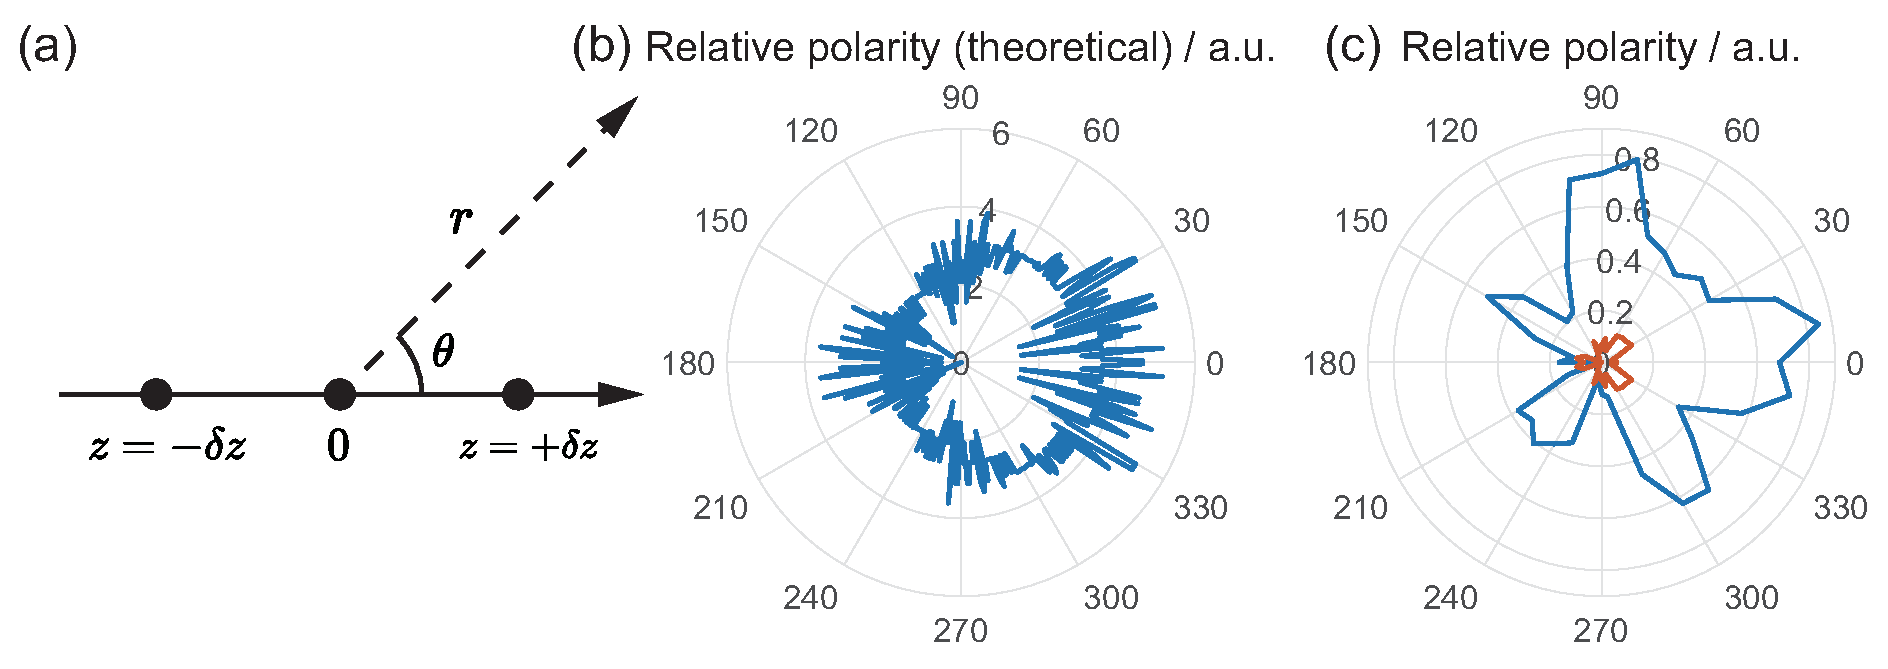
\includegraphics[width=.8\columnwidth]{Phased-Bottle-Array.eps}
    \caption{(a) 声学相控阵装置示意图,$z=0$ 处为小音箱,$z=\pm\delta z$ 处为两组塑料瓶. (b) 理论计算所得相对极化强度,其中 $0^{\circ}$ 代表水位低的塑料瓶一侧,$180^{\circ}$ 代表水位高的塑料瓶一侧(下同). (c) 实验测得,其中蓝色是在塑料瓶盖打开情况下的实验数据,橙色是在塑料瓶盖盖上情况下的实验数据.}
    \label{Phased-Bottle-Array}
\end{figure}

综上,我们测定了塑料瓶在外界气压驱动下的声学响应,其特征与亥姆霍兹共振模型的预测趋势相符;我们以一个十分简单的塑料瓶阵列作为演示,通过加水的方式改变塑料瓶内剩余容积,进而调节塑料瓶在给定外界气压驱动频率下的相位,实现声音的定向传播,证明了声学相控阵的可行性.

\nocite{*}
\bibliographystyle{plain}
\bibliography{References}
\end{document}